% \documentclass{beamer}
\documentclass[xcolor=dvipsnames]{beamer}
\usefonttheme{serif}
%% \usecolortheme[named=Blue]{structure}
\setbeamersize{text margin left=30mm, text margin right=30mm}
\useoutertheme{infolines}
%% \usetheme[height=7mm]{Rochester}
\usetheme{Pittsburgh}
\setbeamertemplate{items}[ball]
\setbeamertemplate{blocks}[rounded][shadow=true]
\setbeamertemplate{navigation symbols}{}

\usepackage[utf8x]{inputenc}
%% \usepackage{default}
\usepackage[english]{babel}
\usepackage{geometry}
%% \usepackage{fullpage}
\usepackage{amsmath, amsthm, amssymb}
\usepackage{listings}
\usepackage{pxfonts}
\usepackage{caption}


\captionsetup[figure]{labelformat=empty}

%% \usepackage{color}
%% \usepackage{graphicx}
%% \usepackage{natbib}
%% \usepackage{array}
%% \usepackage{booktabs}
%% \usepackage{tabu}
%% \usepackage[utf8]{inputenc}
%% \usepackage{fancyhdr}
%% \usepackage{float}
%% \usepackage{subfigure}
%% \usepackage{titlesec}

\setbeamertemplate{headline}{}
\setbeamertemplate{footline}[frame number]{}
\setbeamertemplate{navigation symbols}{}
\setbeamertemplate{footline}{}
\setbeamertemplate{footline}[frame number]

\setbeamertemplate{itemize items}{$-$}

\def\CCT{{C\nolinebreak[4]\hspace{-.05em}\raisebox{.4ex}{\tiny\bf ++}}}
\def\CC{{C\nolinebreak[4]\hspace{-.05em}\raisebox{.4ex}{\small\bf ++}}}


\definecolor{lstgray}{gray}{0.93}
\definecolor{strgray}{gray}{0.4}

\lstset{ %
  escapechar=@,
  language=C++,
  basicstyle=\footnotesize\ttfamily,
  %% basicstyle=\ttfamily,
  %% keywordstyle=\color{blue}\ttfamily,
  keywordstyle=\bfseries,
  stringstyle=\color{strgray}\ttfamily,
  commentstyle=\color{OliveGreen}\ttfamily,
  %% morecomment=[l][\color{red}]{\#},
  morecomment=[l][\color{blue}]{\#},
  backgroundcolor=\color{lstgray},
  %% keywordstyle=\color{red},
  frame=f,
  frameround=ffff,
  tabsize=2,
  breaklines=true,
  breakatwhitespace=false,
  showspaces=false,
  showstringspaces=false,
  xleftmargin=5pt,
  xrightmargin=5pt,
  morekeywords={in,out,ref,auto,inout,import,ushort,scope,exit,mixin,decltype,varid,sizeof,constexpr}
}

\def\redcolor{\color{red}}
\def\bluecolor{\color{blue}}
\def\blackcolor{\color{black}}
\def\graycolor{\color{gray}}
\def\greencolor{\color{OliveGreen}}


\def\sectionname{\translate{Section}}
\def\insertsectionnumber{\arabic{section}}
\setbeamertemplate{section page}
{
  \begin{centering}
    \begin{beamercolorbox}[sep=4pt,center]{part title}
      \usebeamerfont{section title}\insertsection\par
    \end{beamercolorbox}
  \end{centering}
}
\def\sectionpage{\usebeamertemplate*{section page}}


\AtBeginSection{\frame{\sectionpage}}


\title{Transcendentals}
\subtitle{(In the 21\textsuperscript{st} Century)}
\author{Dominic Jones}
\date{\small{August 2019}}
\institute{\small{University of Buckingham}}


\begin{document}


\begin{frame}[plain]
  \titlepage
\end{frame}


\begin{frame}[fragile]{General argument}
  \begin{itemize}
  \item I argue that unity, truth, and goodness are transcendental properties of being, whereas beauty is a \emph{derived} property from these three.\vspace{6mm}
  \item It is when \emph{we} see those three properties shining together in something, we call it \emph{beautiful}.\vspace{5mm}
  \item But to have some idea about transcendentals, first some ideas about \emph{particulars}, \emph{concepts} and \emph{universals} are would be helpful.
  \end{itemize}
\end{frame}


\begin{frame}[fragile]{This talk}
  \begin{itemize}
  \item \textbf{There is a philosophical proof for the existence of pure being.} \vspace{5mm}
  \item Unity is a negation of division; opposed by disintegration. \vspace{2mm}
  \item \emph{(The greatest unity belongs to the most simple being, that without parts.)}\vspace{2mm}
  \item Every being can be known insofar as it is in act; the more actual, the more knowable. \vspace{2mm}
  \item \emph{(Beings have act, not by themselves, but by participation in pure act.)}\vspace{2mm}
  \item The good is what all things desire; to the extent things tend to their perfection they are good. \vspace{2mm}
  \item \emph{(Goodness is the perfection of being. Pure act is perfect being.)}\vspace{2mm}
  \end{itemize}
\end{frame}




\begin{frame}{}
  %% \centering
  \begin{figure}
  \centering
  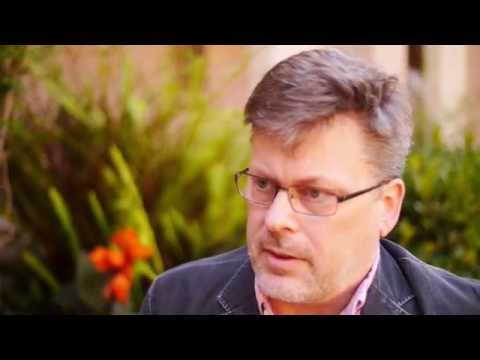
\includegraphics[width=0.6\textwidth]{ed-feser}
\end{figure}
  \begin{quote}
    Abandoning Aristotelianism, as the founders of modern philosophy did, was the single greatest mistake ever made in the entire history of Western thought.
  \end{quote}
      \hspace*{8cm}{Edward Feser}
\end{frame}

\begin{frame}{}
\begin{figure}
  \centering
  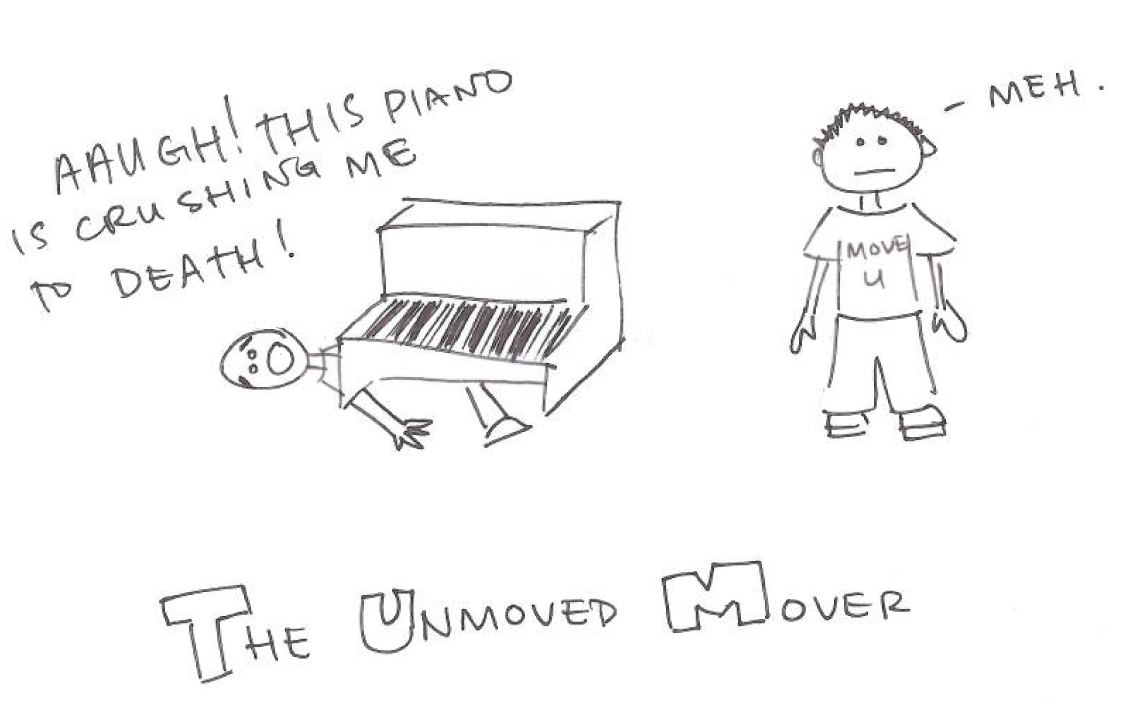
\includegraphics[width=0.99\textwidth]{unmoved_mover}
\end{figure}
\end{frame}


\section{Premise 1: At least something changes}


\begin{frame}{From becoming cold or fat\ldots}
\begin{figure}
  \centering
  \begin{columns}
    \column{0.5\textwidth}
    \centering
    \caption {Qualitative change}
    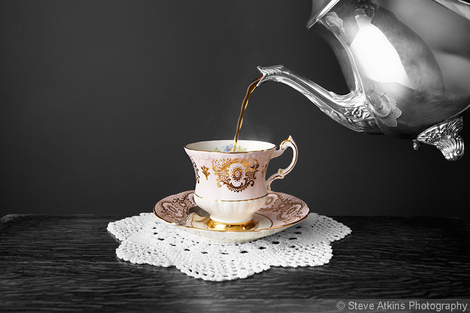
\includegraphics[width=0.99\textwidth]{tea}
    \column{0.5\textwidth}
    \centering
    \caption {Quantitative change}
    
\includegraphics[width=0.99\textwidth]{cat}
  \end{columns}
\end{figure}
\end{frame}

\begin{frame}{or to dropping and dying\ldots}
\begin{figure}
  \centering
  \begin{columns}
    \column{0.5\textwidth}
    \centering
    \caption {Change of location}
    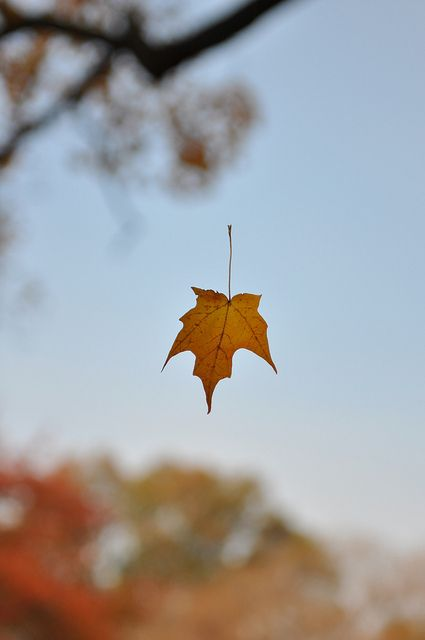
\includegraphics[width=0.99\textwidth]{leaf}
    \column{0.5\textwidth}
    \centering
    \caption {Substantial change}
    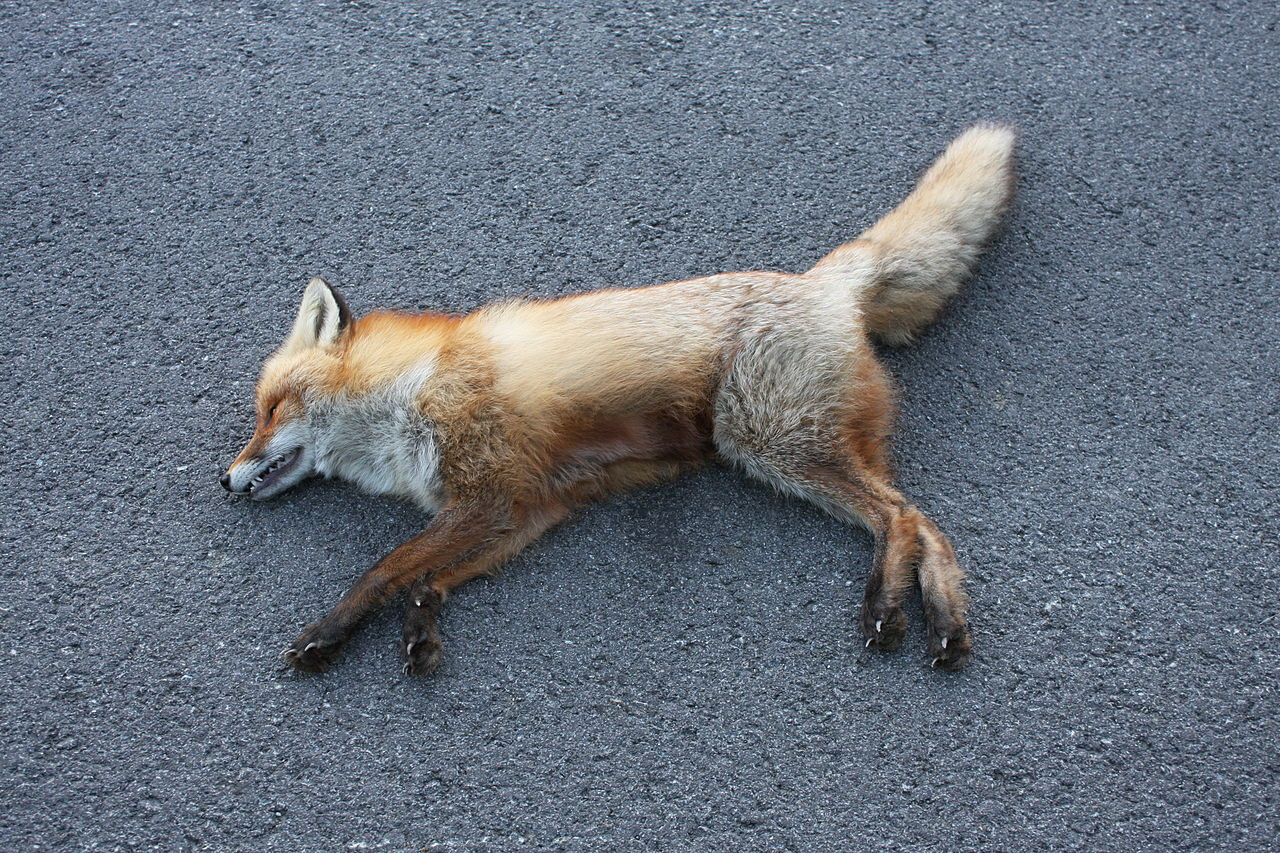
\includegraphics[width=0.99\textwidth]{fox}
  \end{columns}
\end{figure}
\end{frame}

\begin{frame}{or going from ignorance to knowledge}
\begin{figure}
  \centering
  \begin{columns}
    \column{0.5\textwidth}
    \centering
    \caption {Change of mind}
    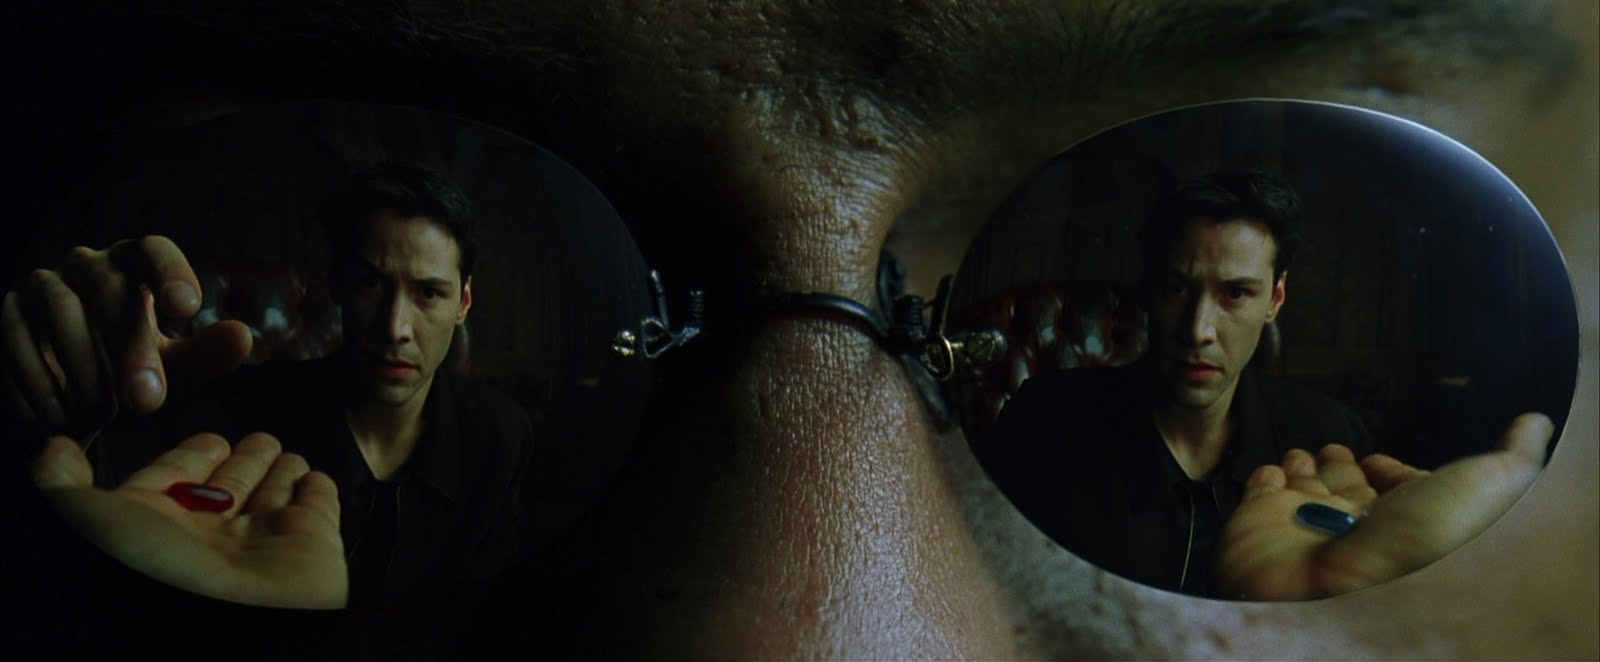
\includegraphics[width=0.99\textwidth]{pills}
    \column{0.5\textwidth}
    \centering
    \caption {Casting doubt}
    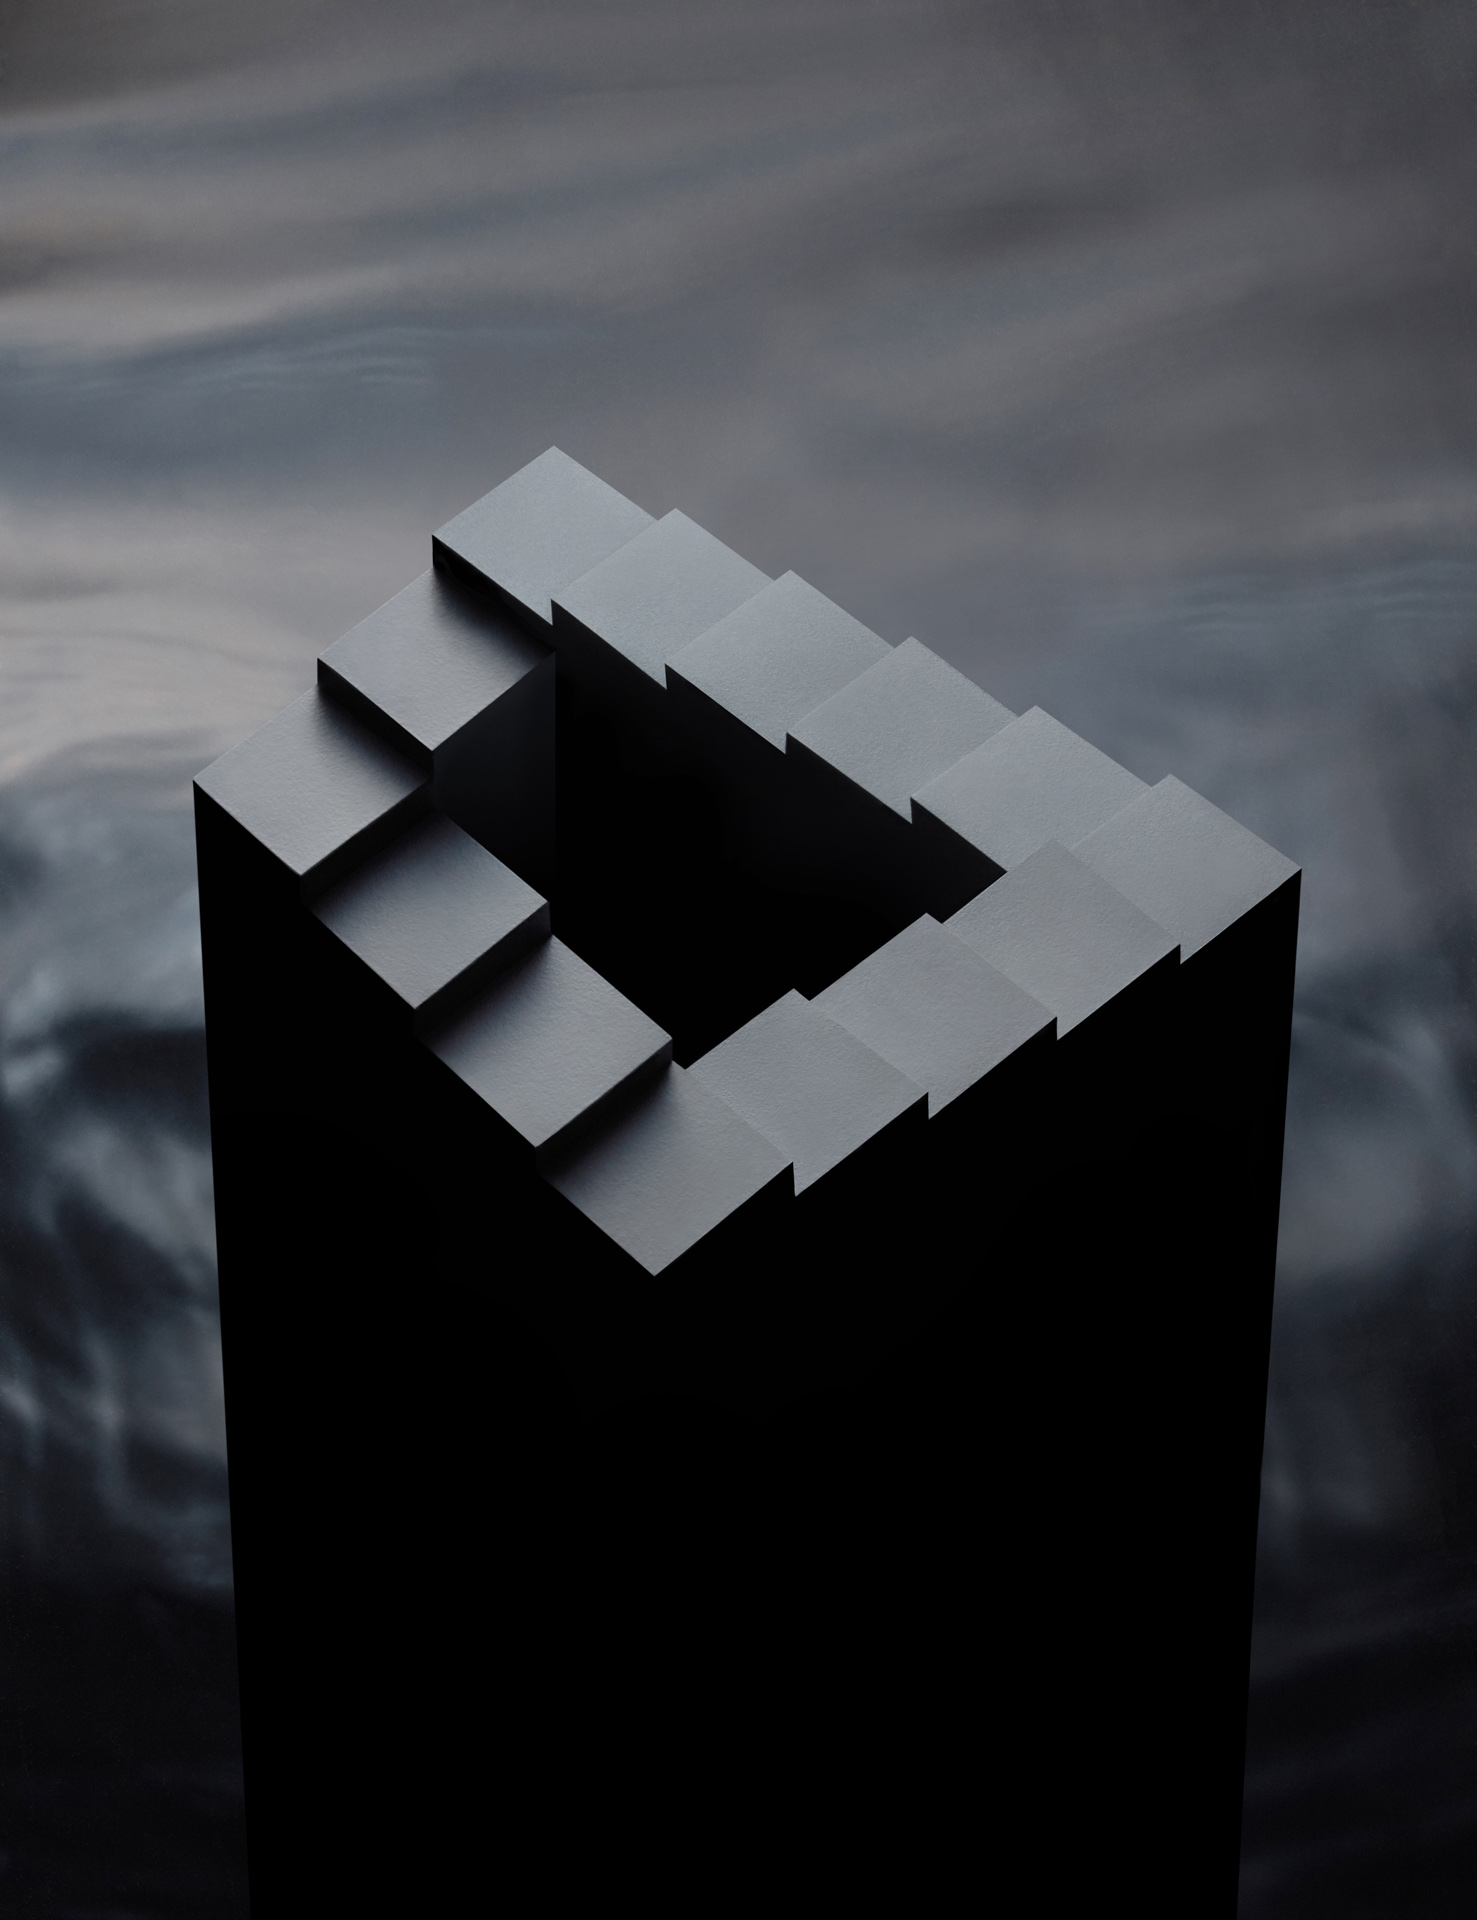
\includegraphics[width=0.99\textwidth]{stairs}
  \end{columns}
\end{figure}
\end{frame}


\begin{frame}[fragile]{Change}
  \begin{itemize}
  \item There is at least some change in something. \vspace{5mm}
  \item To undergo some change, the actual thing being changed must in some way be in potential the thing it becomes. \vspace{5mm}
  \item Things that may change are at once actually something but also potentially something else. \vspace{5mm}
  \item A thing that changes cannot change exclusively by itself. \vspace{5mm}
  \end{itemize}
\end{frame}


\section{Premise 2: A change needs a changer}


\begin{frame}{}
\begin{figure}
  \centering
  \begin{columns}
    \column{0.5\textwidth}
    \centering
    \caption {This can be many things\ldots}
    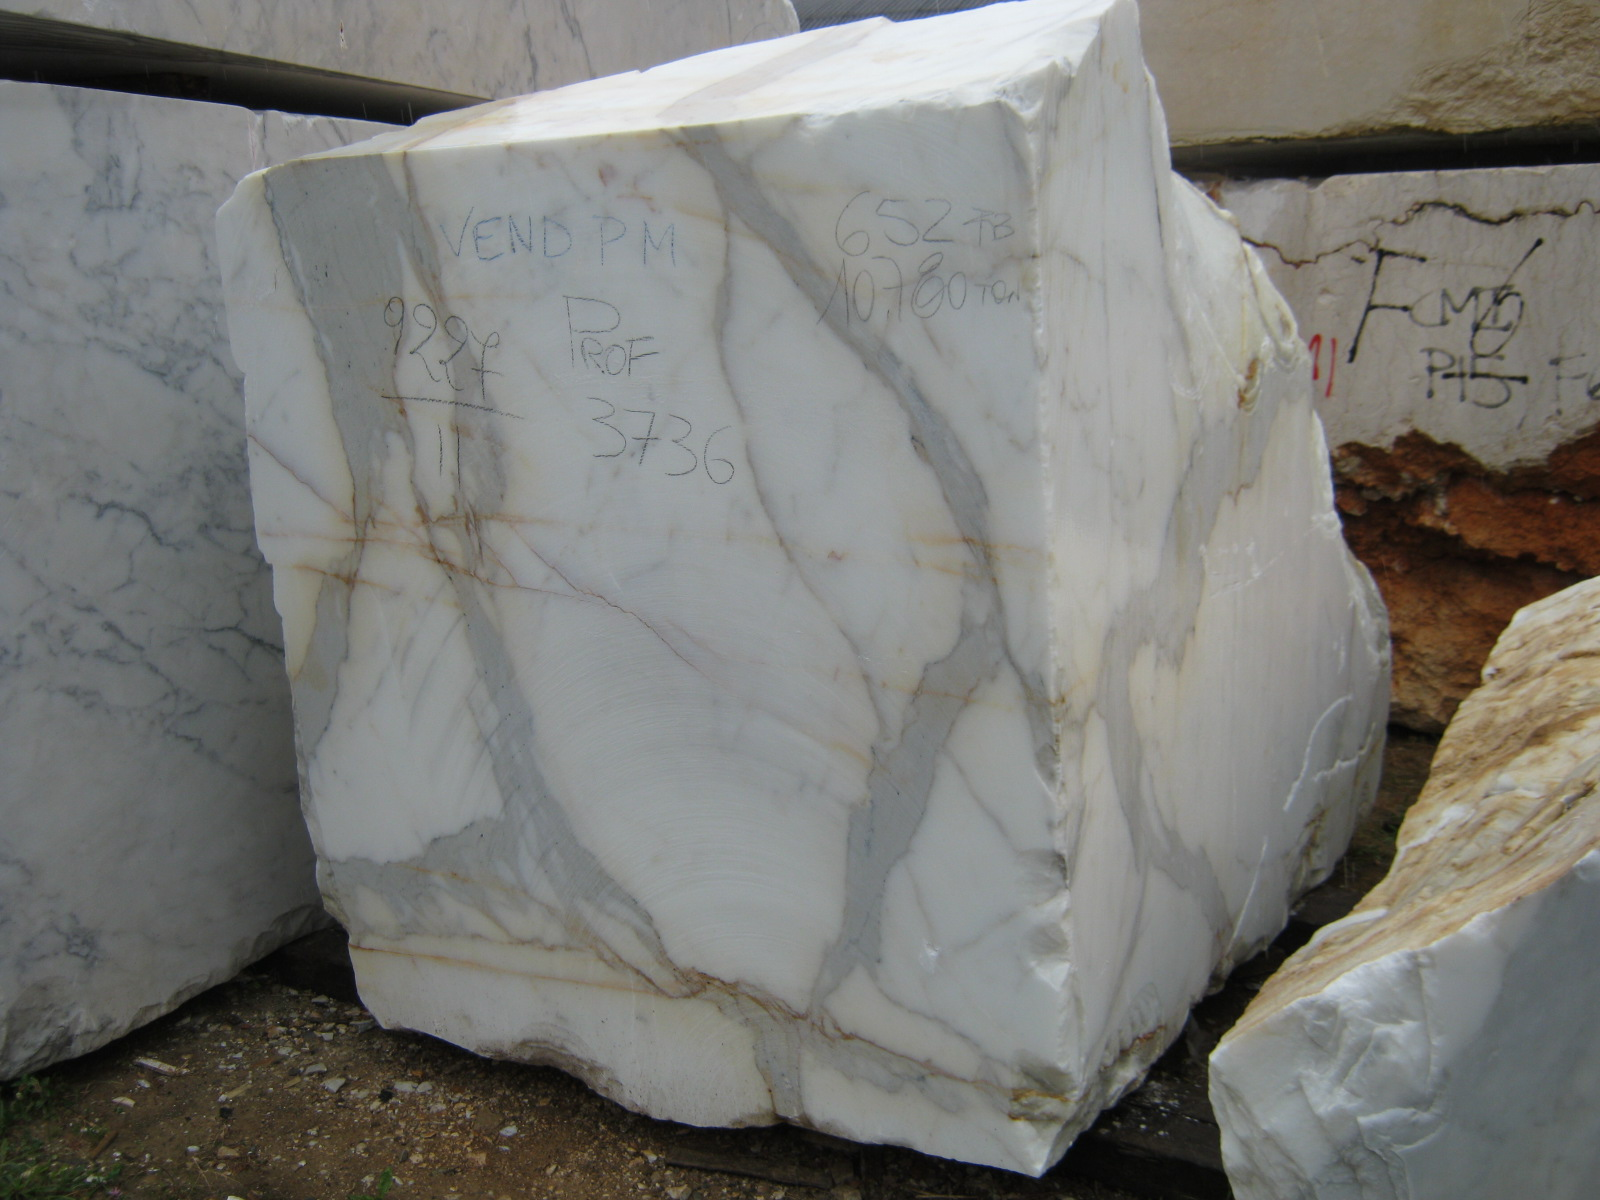
\includegraphics[width=0.99\textwidth]{marble}
    \column{0.5\textwidth}
    \centering
    \caption {through an agent of change}
    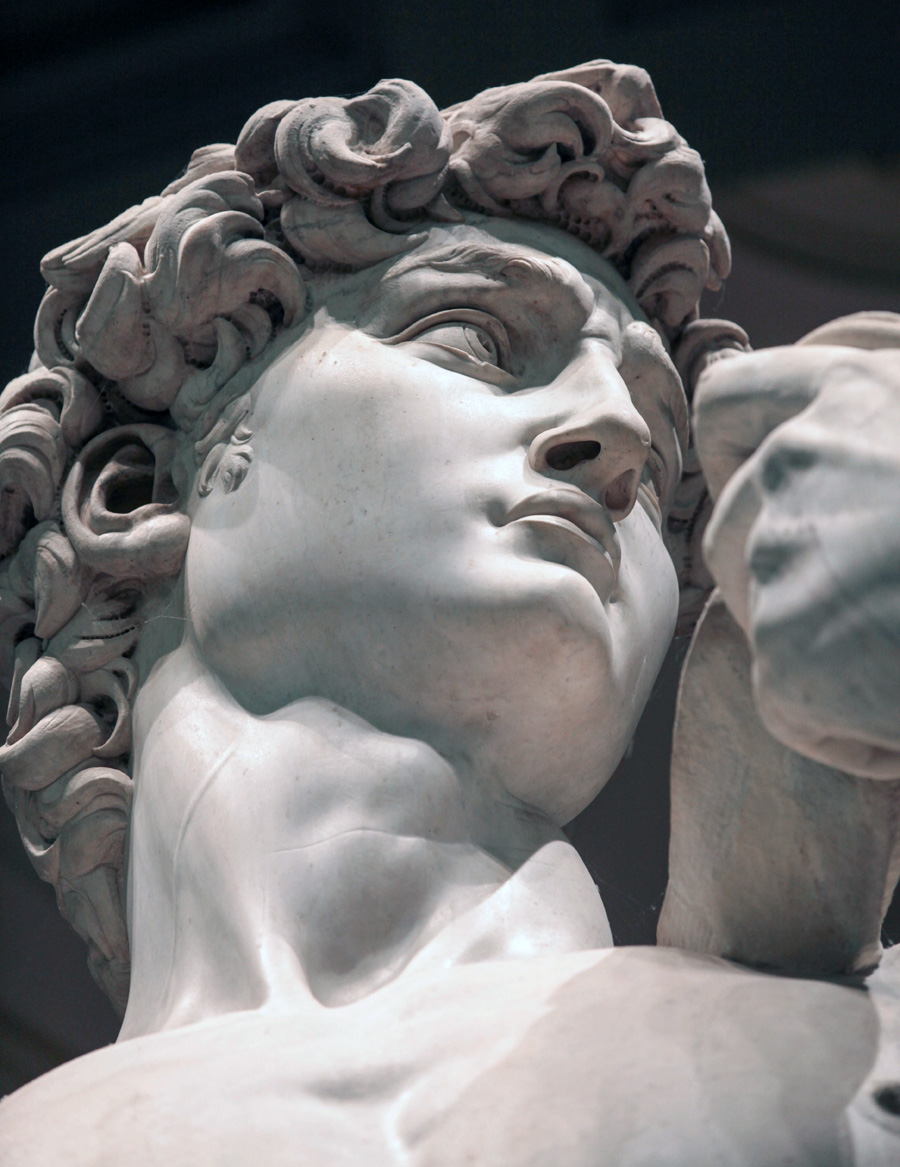
\includegraphics[width=0.99\textwidth]{david}
  \end{columns}
\end{figure}
\end{frame}

\begin{frame}[fragile]{Agent}
  \begin{itemize}
  \item Potential `David' cannot make itself, therefore an agent of change is required. \vspace{5mm}
  \item That agent must be actual to bring about the change, therefore what is actual is \emph{prior} to what is potential. \vspace{5mm}
    \item This kind of \emph{linear} change could go on forever\ldots \vspace{5mm}
  \end{itemize}
\end{frame}

\begin{frame}{\ldots or could go back forever}
\begin{figure}
  \centering
  \begin{columns}
    %% \column{0.5\textwidth}
    %% \centering
    %% \caption {Can be many things...}
    %% 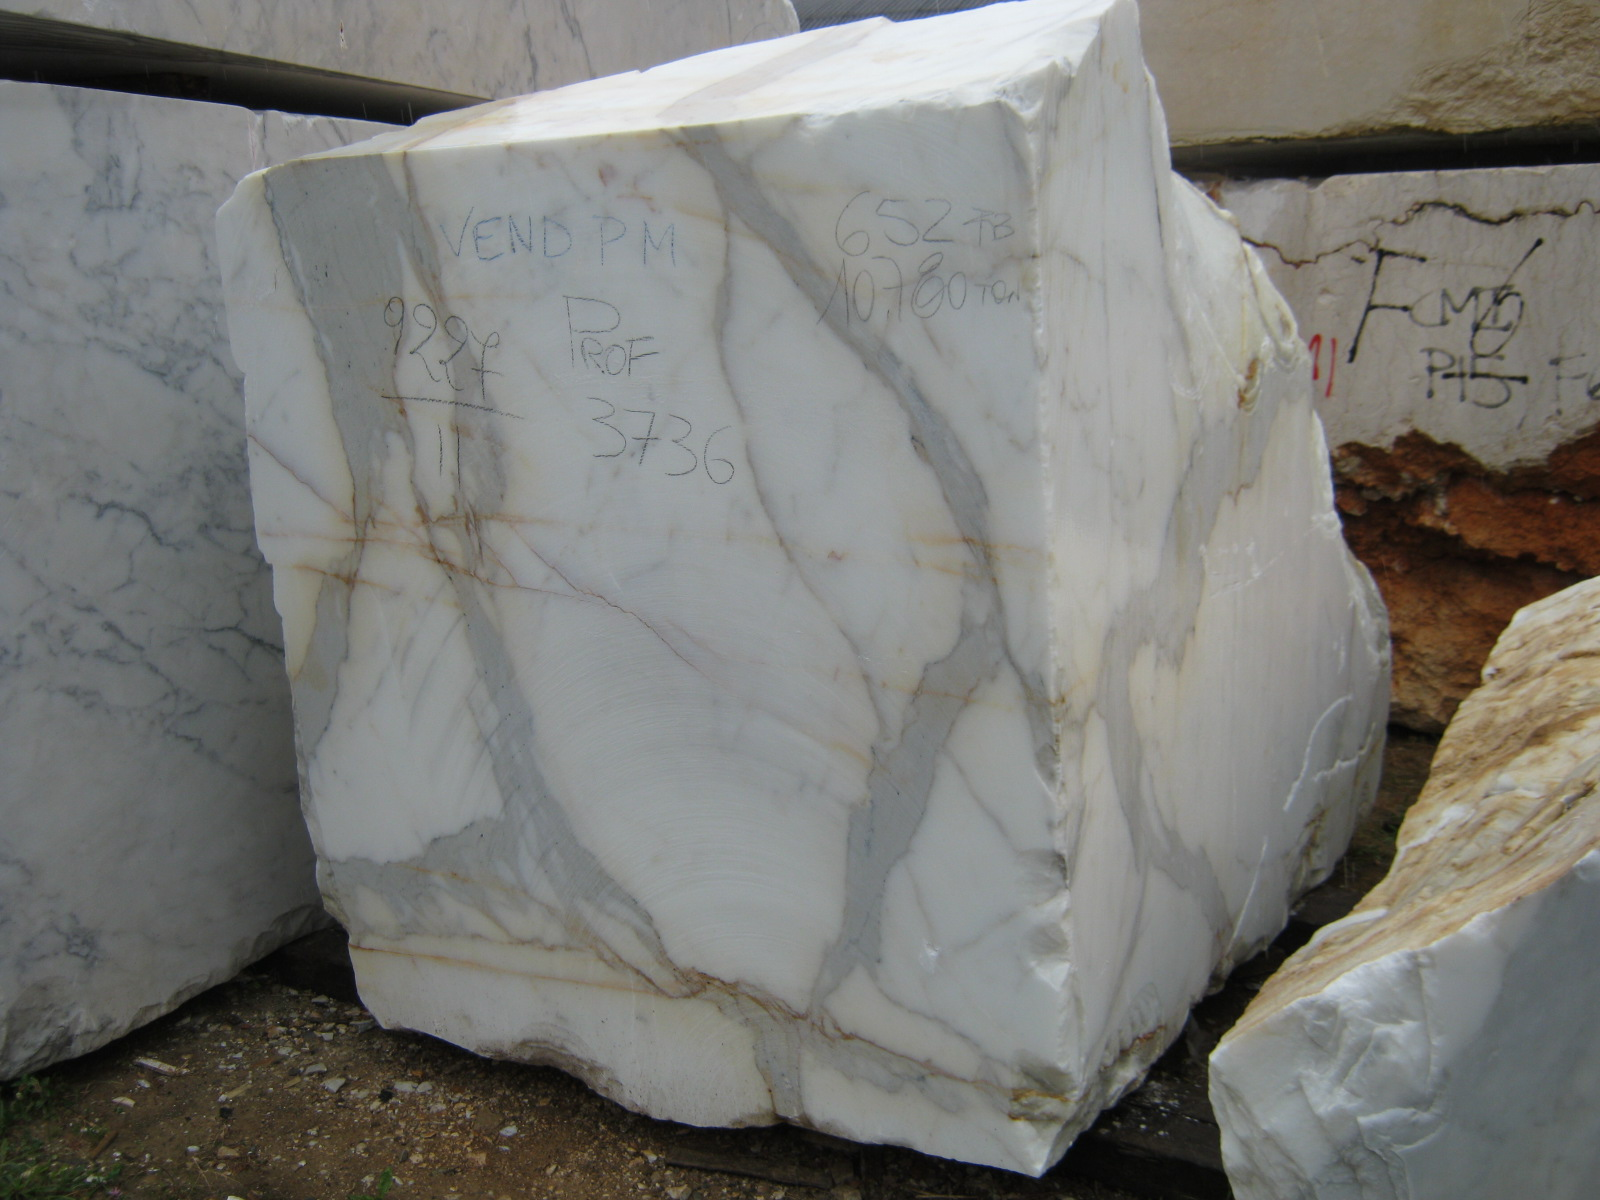
\includegraphics[width=0.99\textwidth]{marble}
    \column{0.99\textwidth}
    \centering
    %% \caption {(but this is irrelevant)}
    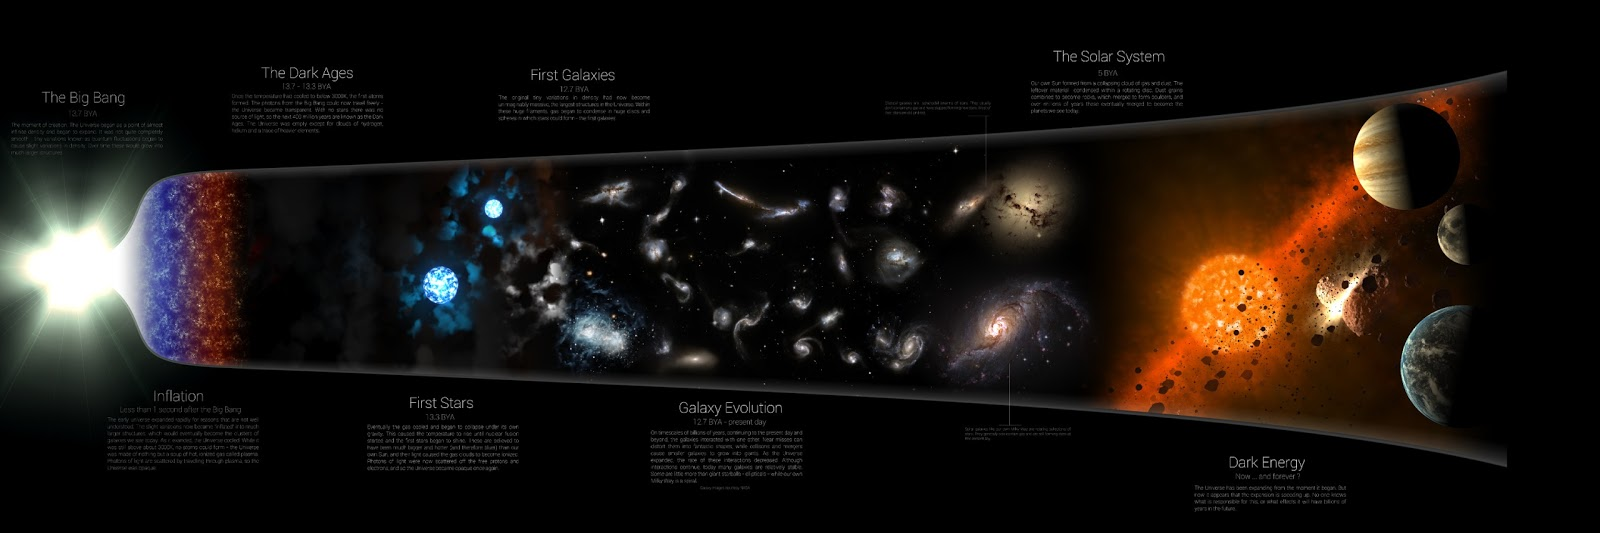
\includegraphics[width=0.99\textwidth]{big_bang}
  \end{columns}
\end{figure}
  \begin{itemize}
  \item Changes in time could \emph{metaphysically} have no starting point (no first member). \vspace{5mm}
  \item A linear series of changes is not \emph{at once} hierarchically dependent. \vspace{5mm}
  \end{itemize}
\end{frame}


\section{Step 1: hierarchical change}


\begin{frame}[fragile]{Hierarchy of the actual}
  \begin{itemize}
  \item Things that change are described as having potency and act. \vspace{5mm}
  \item But something that can change, and is the way it is \emph{here and now}, is also the actualisation of a potential. \vspace{5mm}
    \item This kind of change is hierarchical: if there is no inherent power to be the way it is, this power must be derived.
  \end{itemize}
\end{frame}

\begin{frame}{An instrument of real power}
\begin{figure}
  \centering
  \begin{columns}
    \column{0.5\textwidth}
    \centering
    \caption {Impossible!}
    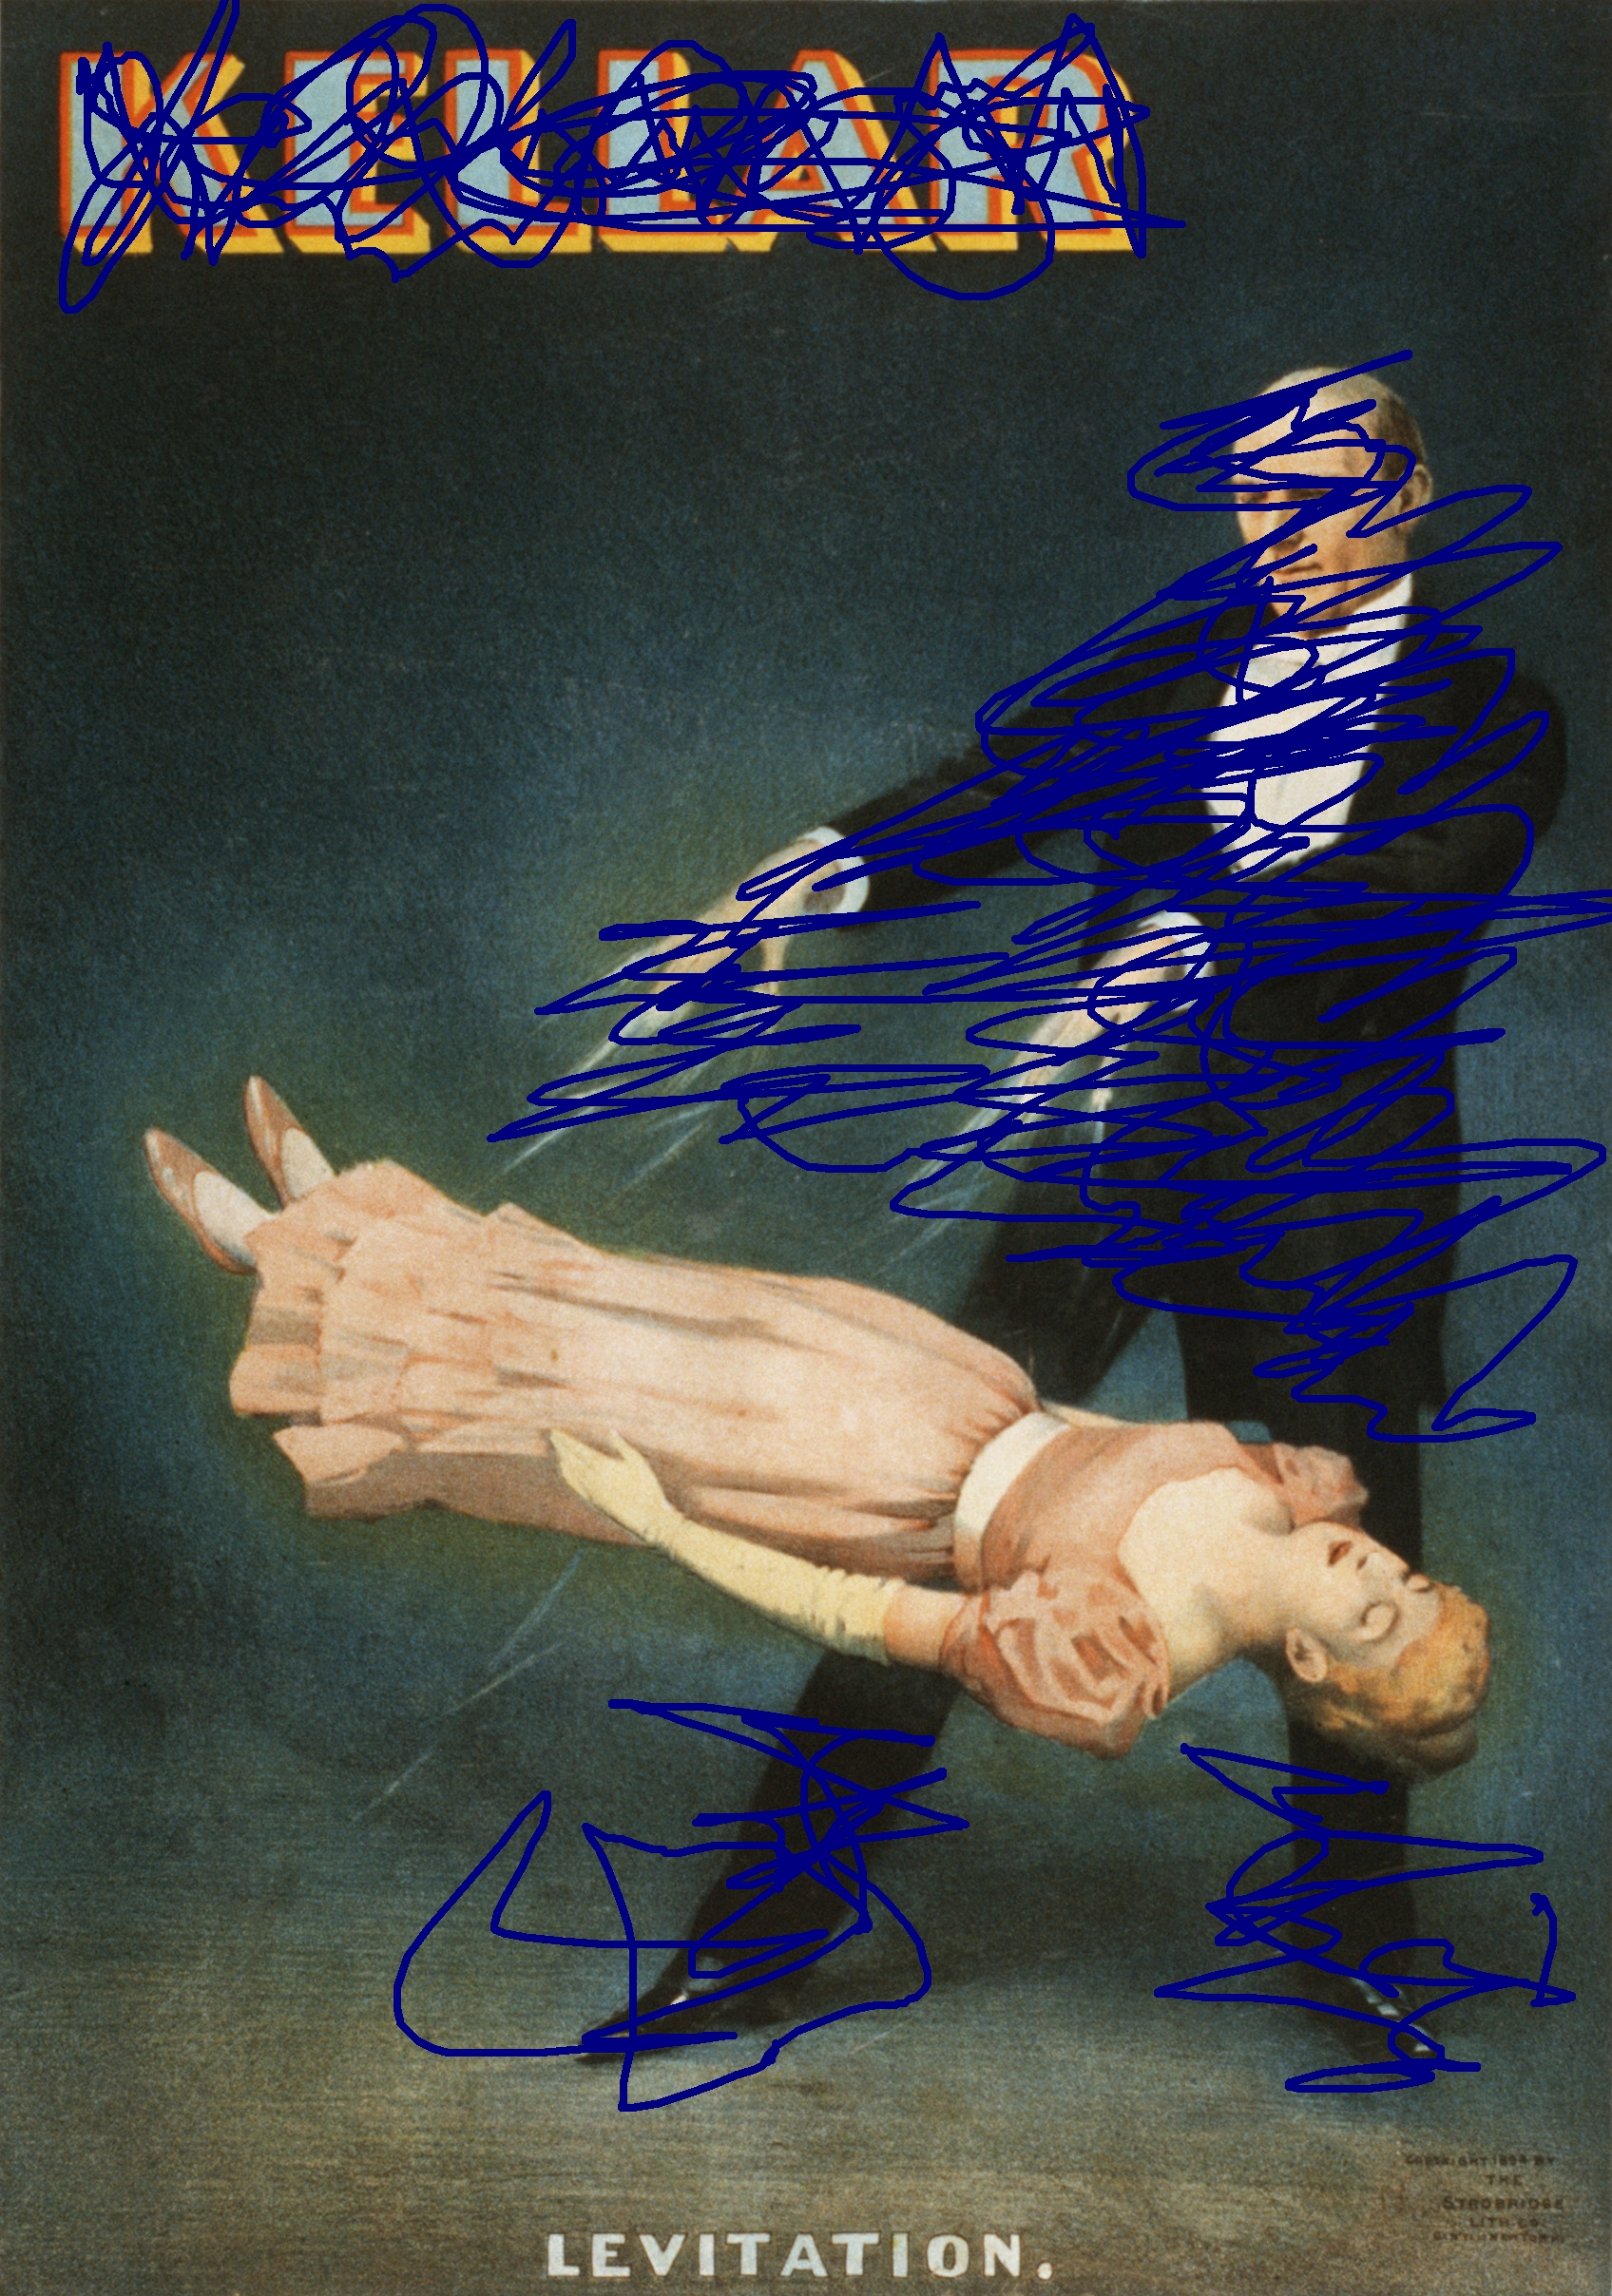
\includegraphics[width=0.99\textwidth]{levitation2}
    \column{0.5\textwidth}
    \centering
    \caption {An everyday occurrence}
    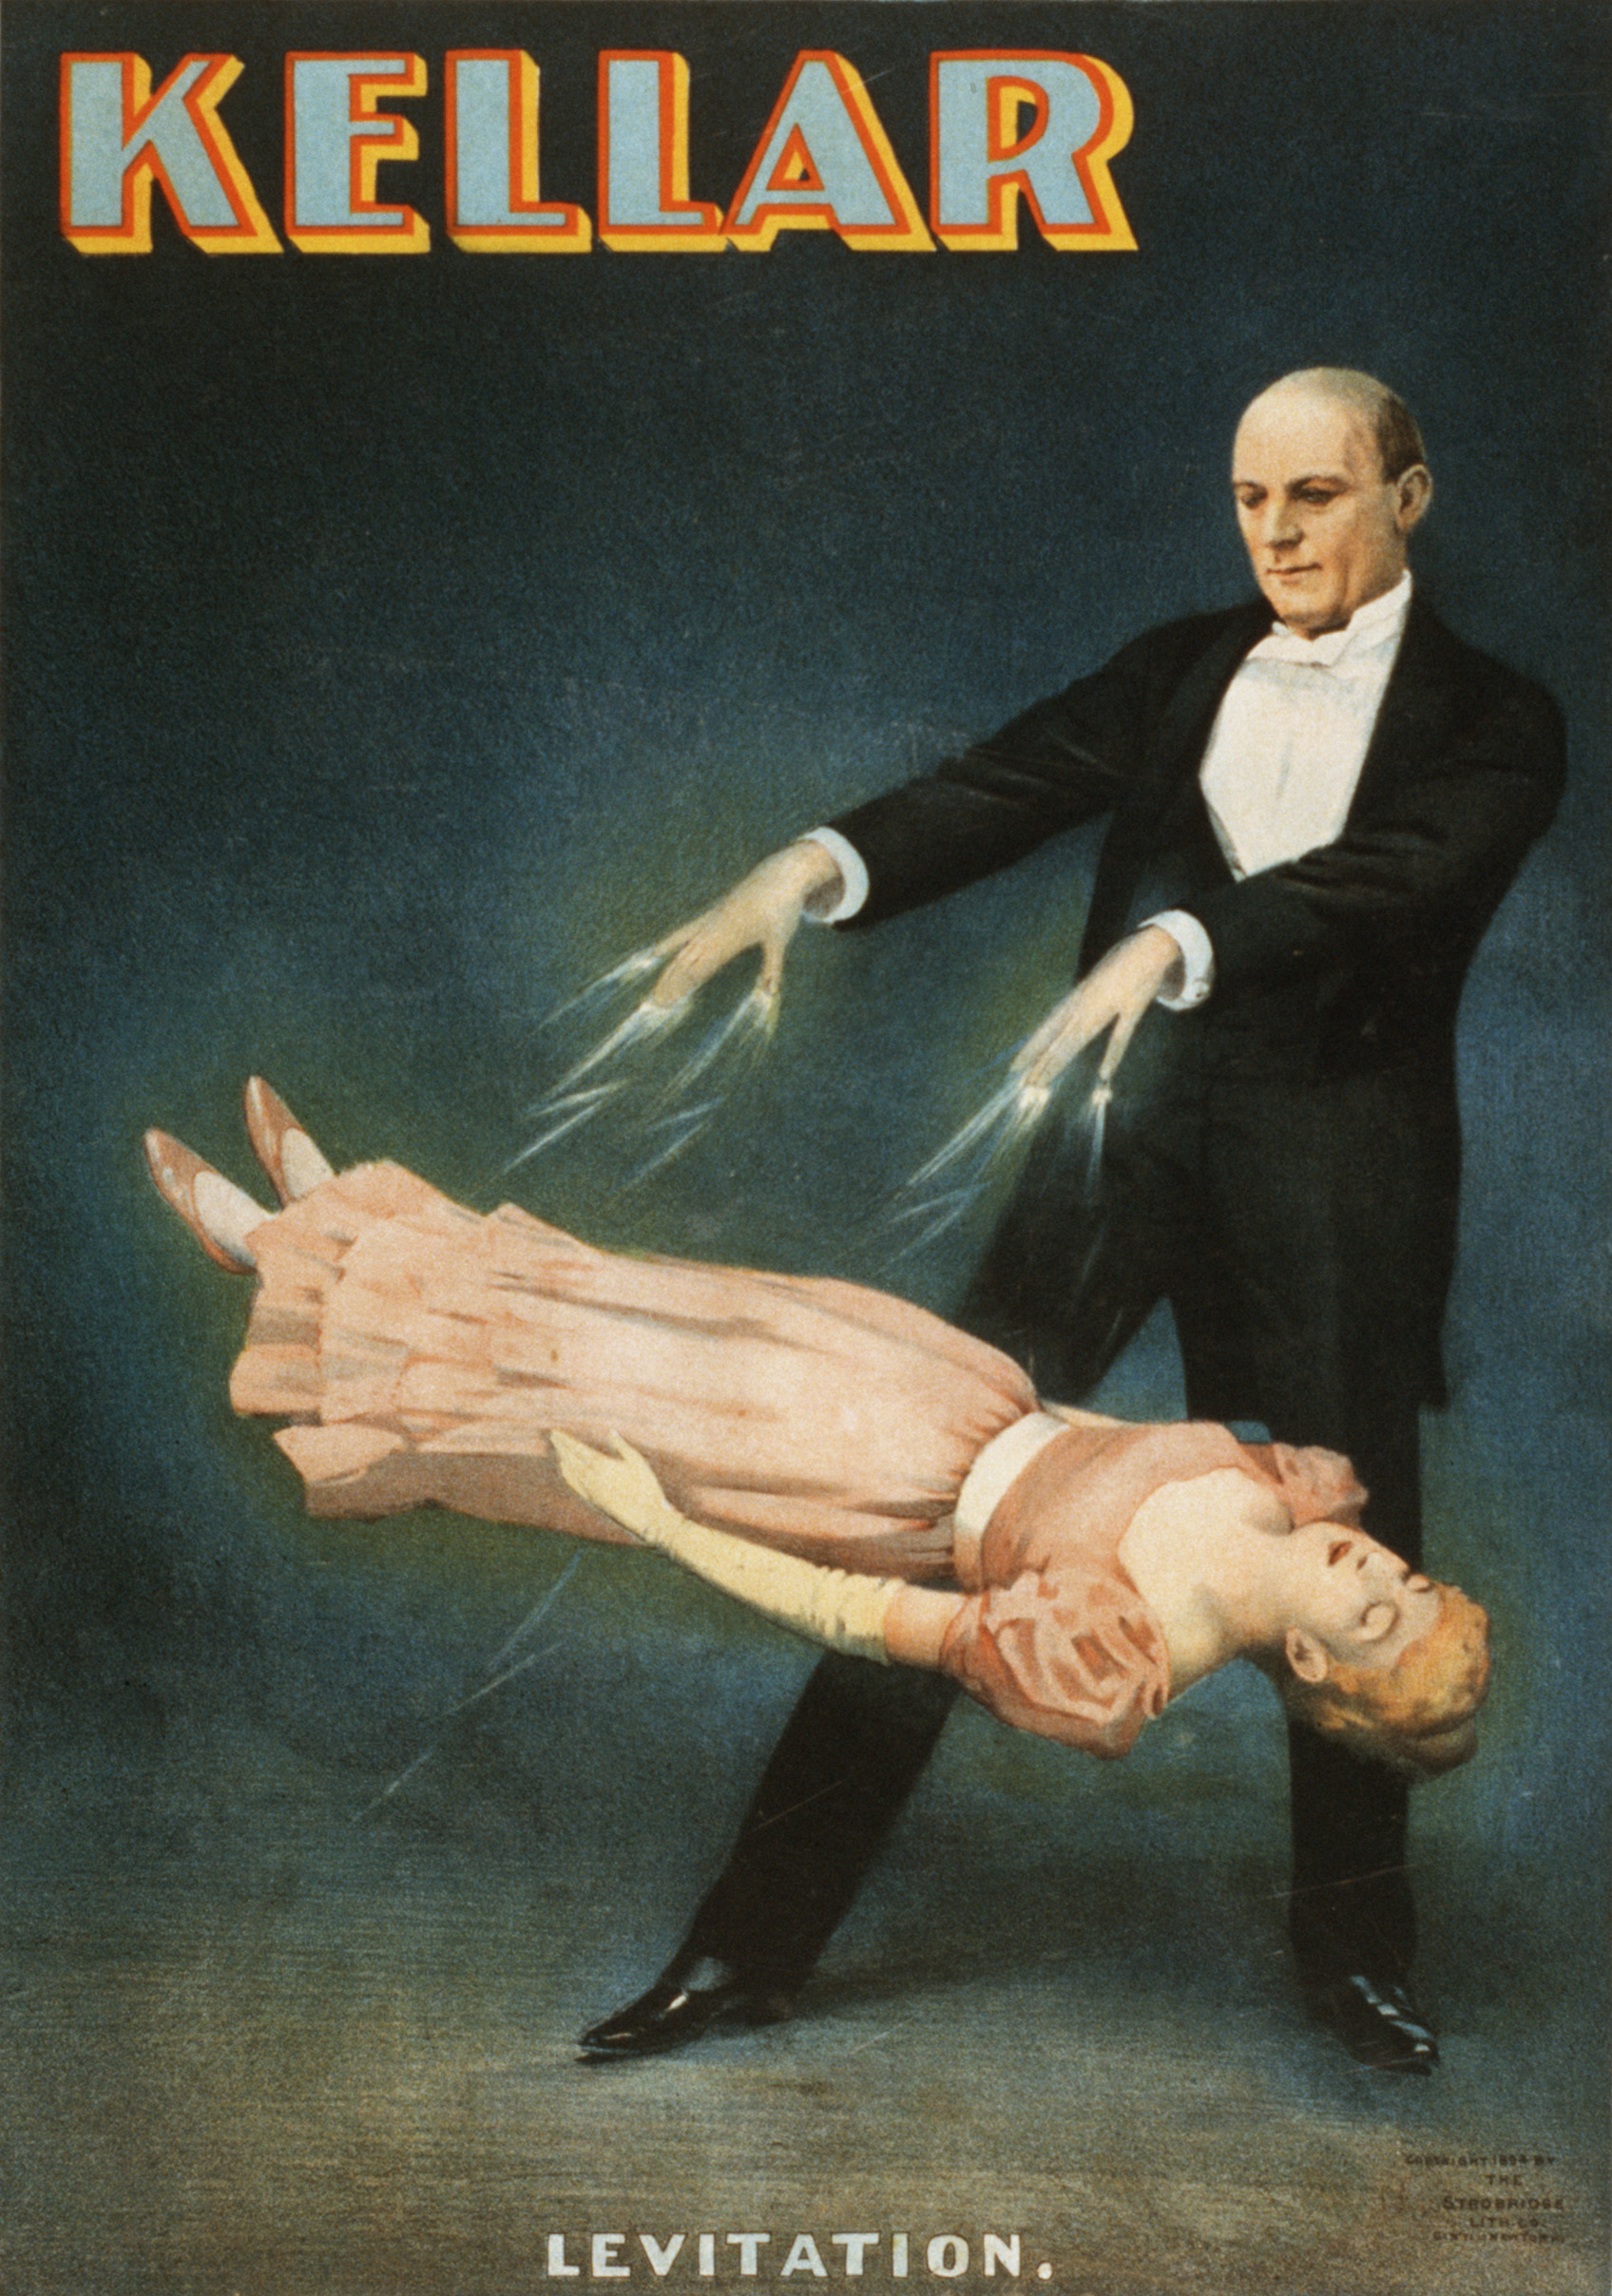
\includegraphics[width=0.99\textwidth]{levitation}
  \end{columns}
\end{figure}
\end{frame}


\begin{frame}[fragile]{First in line}
  \begin{itemize}
  \item She cannot hold herself in the air by herself. \vspace{5mm}
  \item The power to do so is imparted through the great `Kellar', despite being \emph{merely} an instrument. \vspace{5mm}
  \item She is \emph{potentially} flat on the ground but for the \emph{act} of the intermediary. \vspace{5mm}
  \item But not `and so on forever': something \emph{actual} must terminate this imparted power. \vspace{5mm}
  \end{itemize}
\end{frame}


\section{Step 2: Something that changes must first exist}


\begin{frame}{(But not everything can change)}
\begin{figure}
  \centering
  \begin{columns}
    \column{0.4\textwidth}
    \centering
    \caption {Object of thought (abstract)}
    
\includegraphics[width=0.99\textwidth]{number}
    \column{0.6\textwidth}
    \centering
    \caption {Object of some people's thought}
    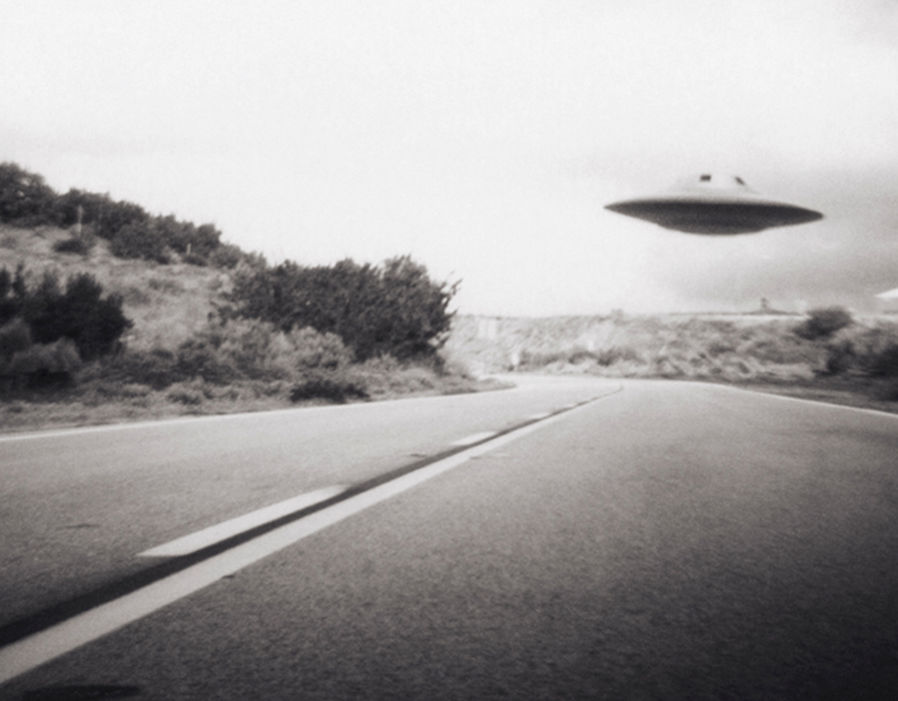
\includegraphics[width=0.99\textwidth]{ufo}
  \end{columns}
\end{figure}
\end{frame}


\begin{frame}[fragile]{Hierarchy of being}
  \begin{itemize}
  \item Change can happen only if the thing exists. \vspace{5mm}
  \item But what keeps the thing in existence \emph{here and now}? \vspace{5mm}
  \item How something \emph{came to be} or how it might \emph{cease to exist} would not answer the question. \vspace{5mm}
  \end{itemize}
\end{frame}


\begin{frame}{Only `To Be' imparts being}
\begin{figure}
  \centering
  \begin{columns}
    %% \column{0.5\textwidth}
    %% \centering
    %% \caption {Can be many things...}
    %% 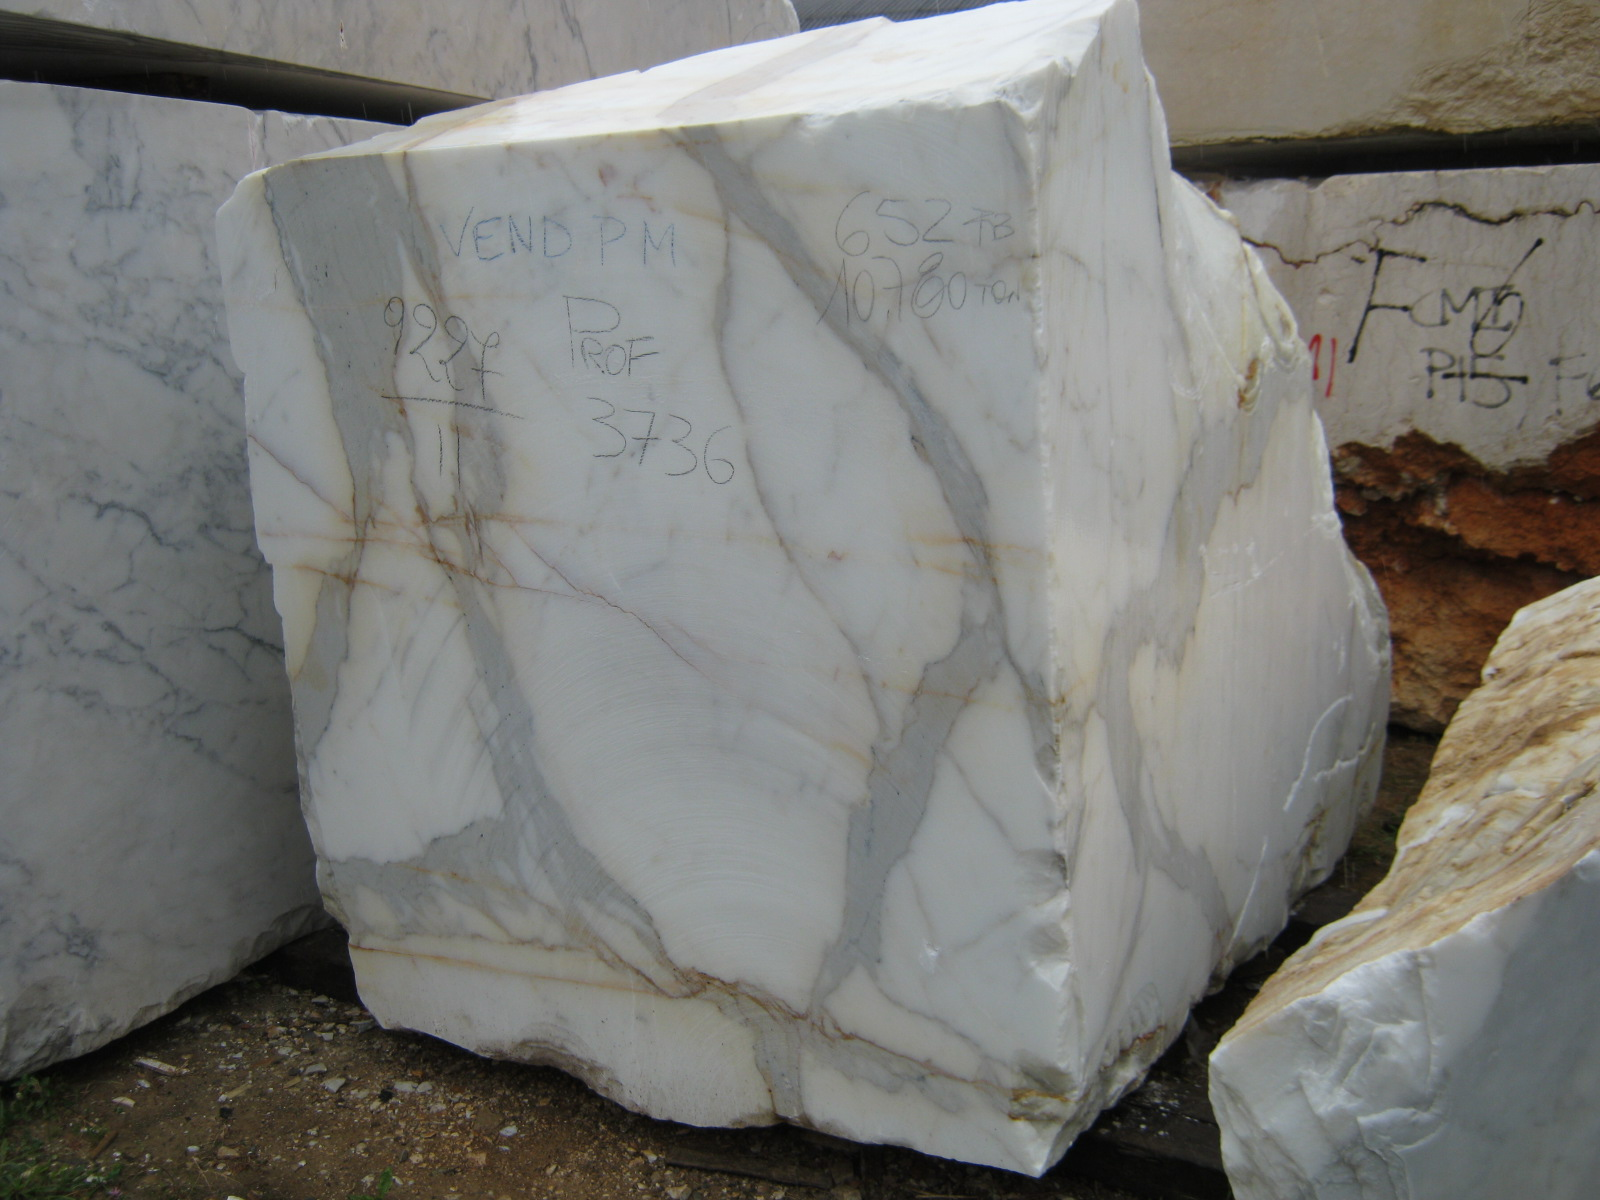
\includegraphics[width=0.99\textwidth]{marble}
    \column{0.99\textwidth}
    \centering
    %% \caption {(but this is irrelevant)}
    
\includegraphics[width=0.99\textwidth]{to_be}
  \end{columns}
\end{figure}
\end{frame}

\begin{frame}[fragile]{\emph{The} Unactualised Actualiser}
  \begin{itemize}
  \item The first cause of existence must have no potential for existence. \vspace{5mm}
  \item Pure actuality, then, could not have a cause of its own nor can it change. \vspace{5mm}
  \item Time is a measure of change --- therefore not in time. \vspace{5mm}
  \item To be material entails being changeable --- therefore not material. \vspace{5mm}
  \item \ldots and other attributes, such as\ldots
  \end{itemize}
\end{frame}


\section{Step 3: Intelligent, of the omniscient kind}


\begin{frame}{There's more to this{\ldots}}
\begin{figure}
  \centering
  \begin{columns}
    %% \column{0.5\textwidth}
    %% \centering
    %% \caption {Can be many things...}
    %% 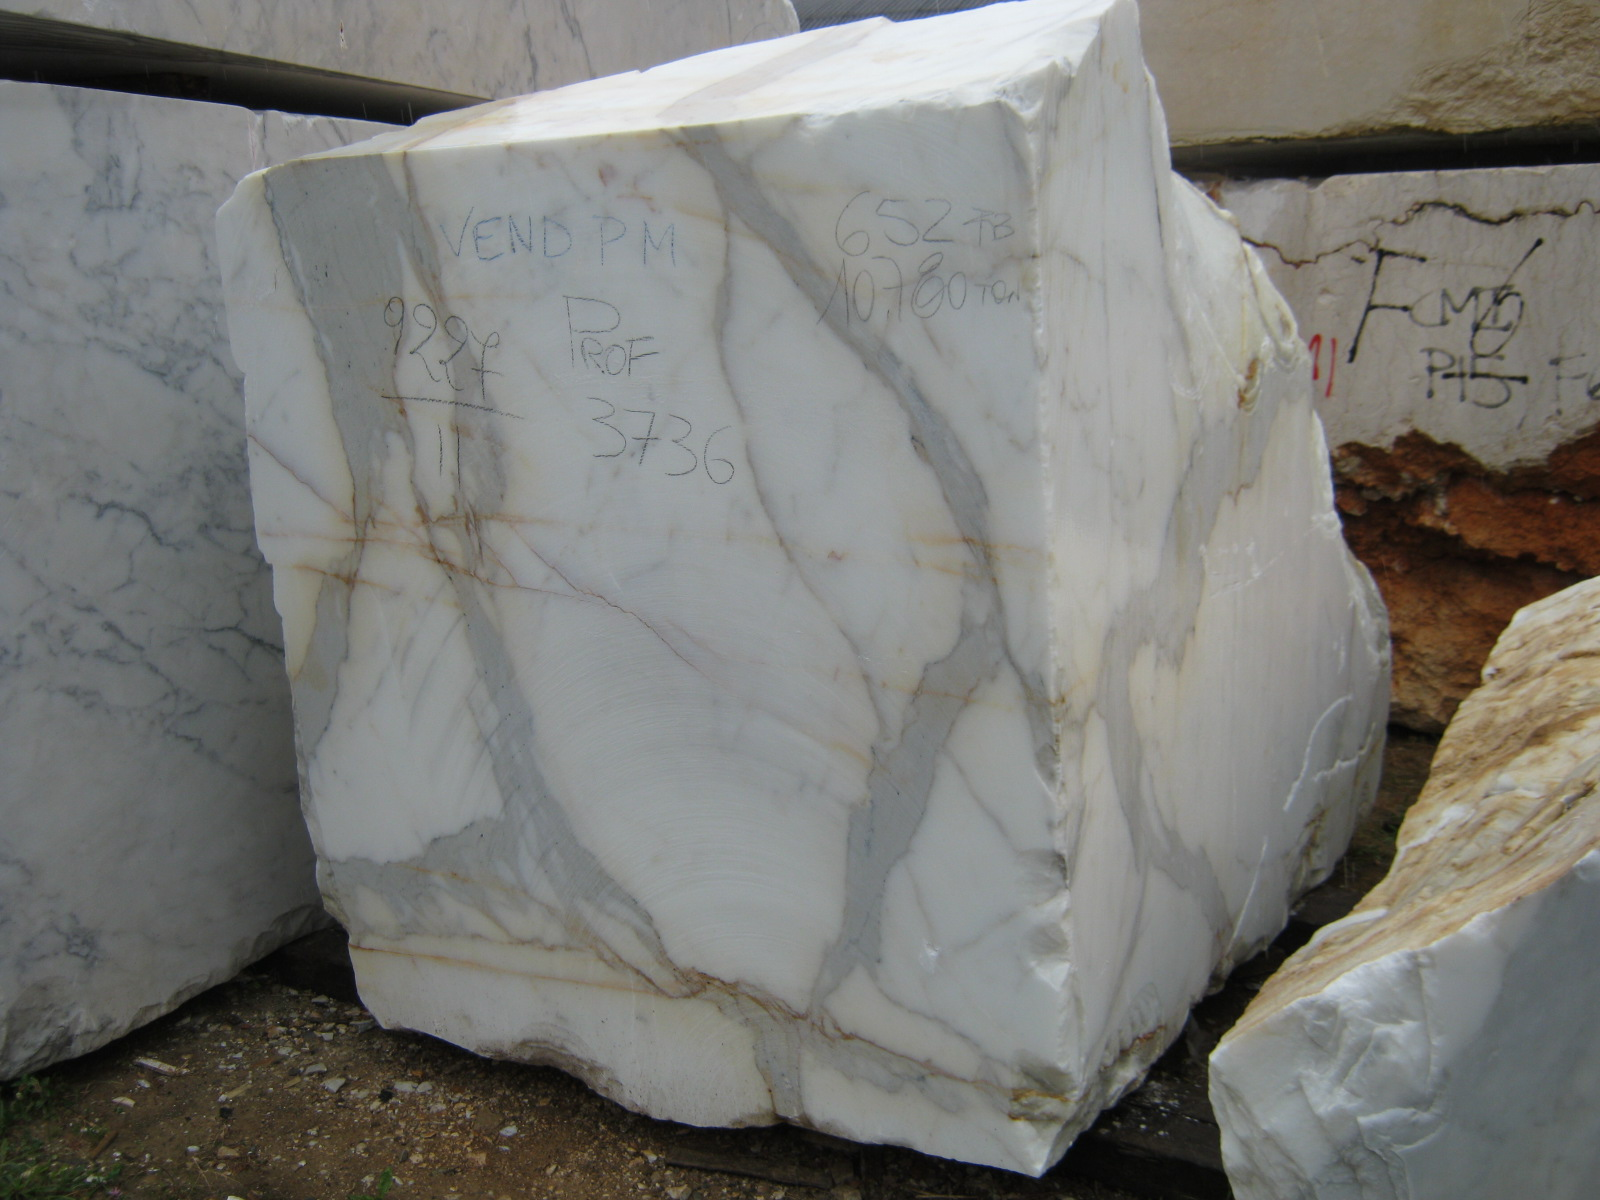
\includegraphics[width=0.99\textwidth]{marble}
    \column{0.99\textwidth}
    \centering
    %% \caption {(but this is irrelevant)}
    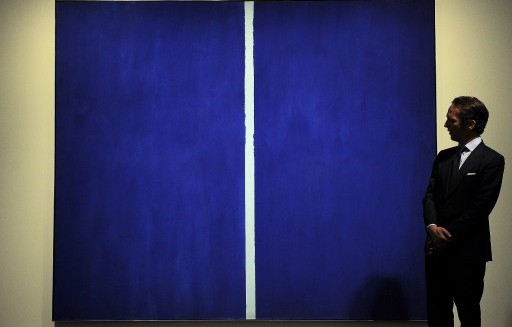
\includegraphics[width=0.99\textwidth]{abstract}
  \end{columns}
\end{figure}
\end{frame}


\begin{frame}[fragile]{Before it was painted, it was thought}
  \begin{itemize}
  \item Intelligence entails at least knowing the \emph{form} of things, i.e. what things are essentially. \vspace{5mm}
  \item Whatever is in an effect, must in some way be in the totality of its cause. \vspace{5mm}
  \item The cause of a thing's existence must also be the cause of the form of its existence. \vspace{5mm}
  \item And so too for all that is. \vspace{5mm}
  \end{itemize}
\end{frame}


\section{Step 4: Less than good entails a privation}


\begin{frame}{But, not all goods are competitive}
\begin{figure}
  \centering
  \begin{columns}
    %% \column{0.5\textwidth}
    %% \centering
    %% \caption {Can be many things...}
    %% 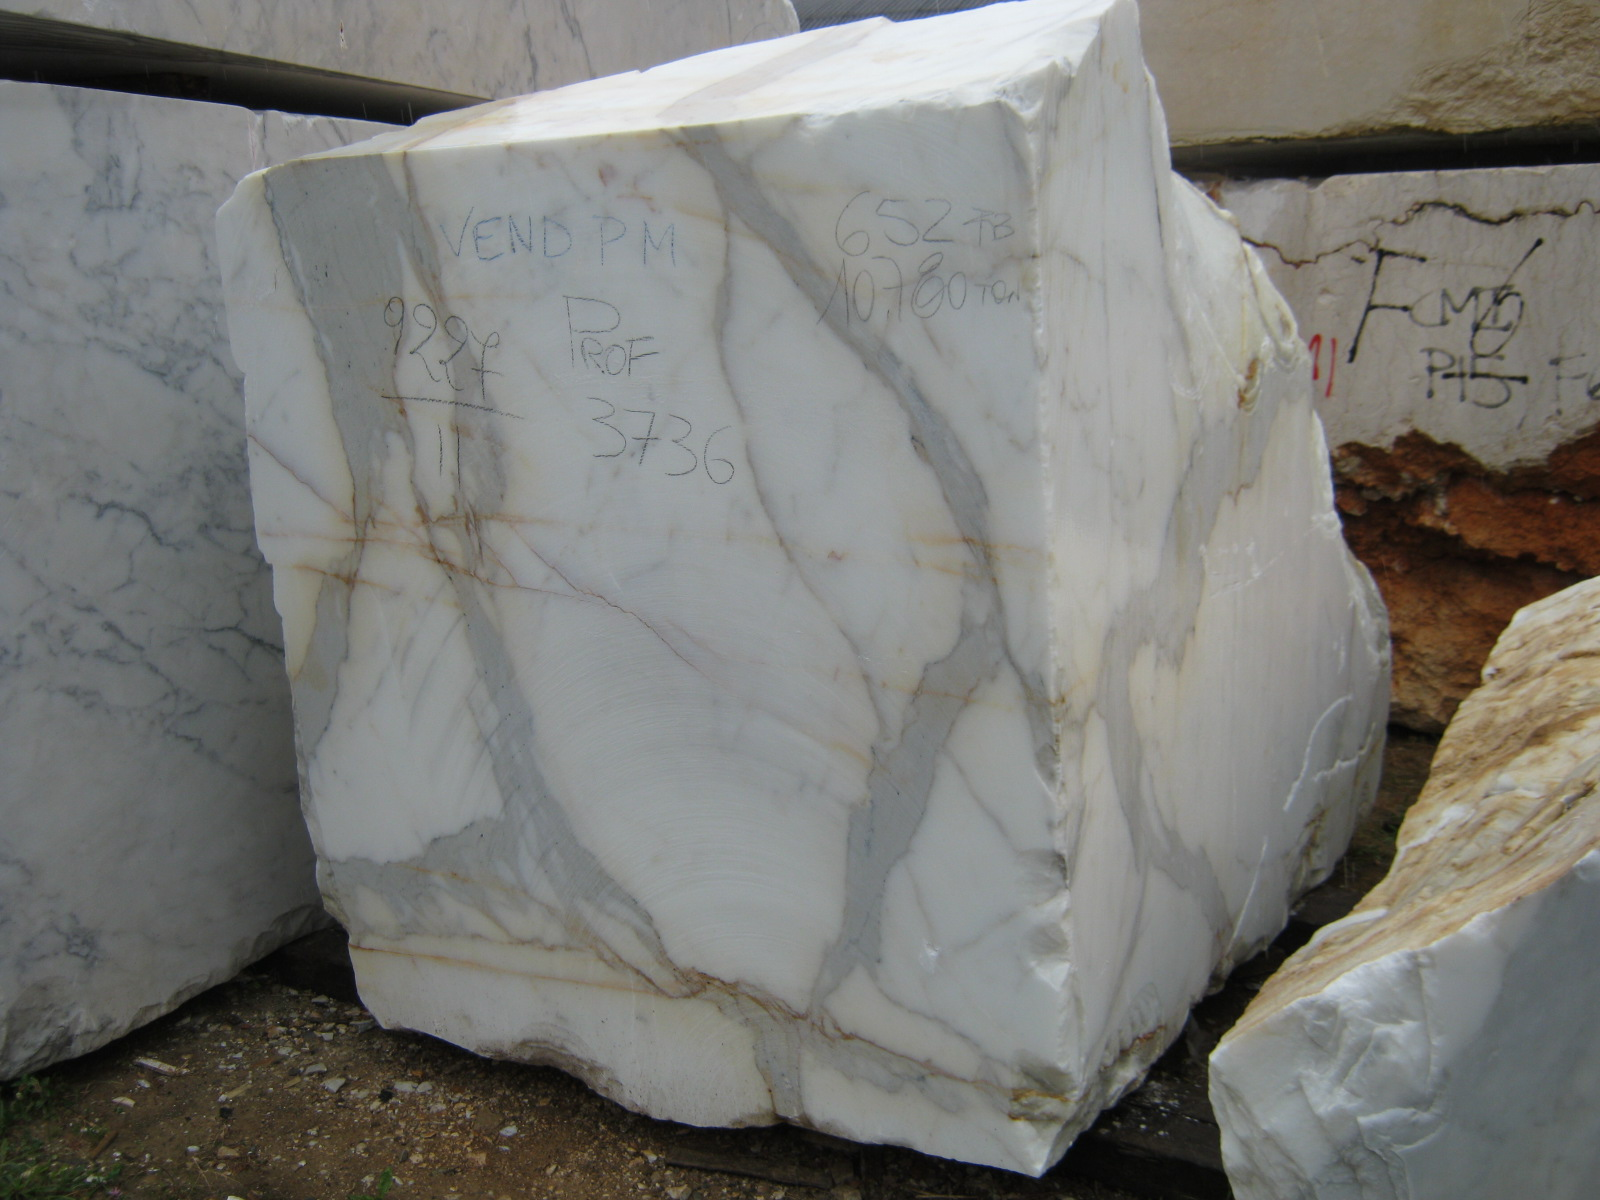
\includegraphics[width=0.99\textwidth]{marble}
    \column{0.99\textwidth}
    \centering
    %% \caption {(but this is irrelevant)}
    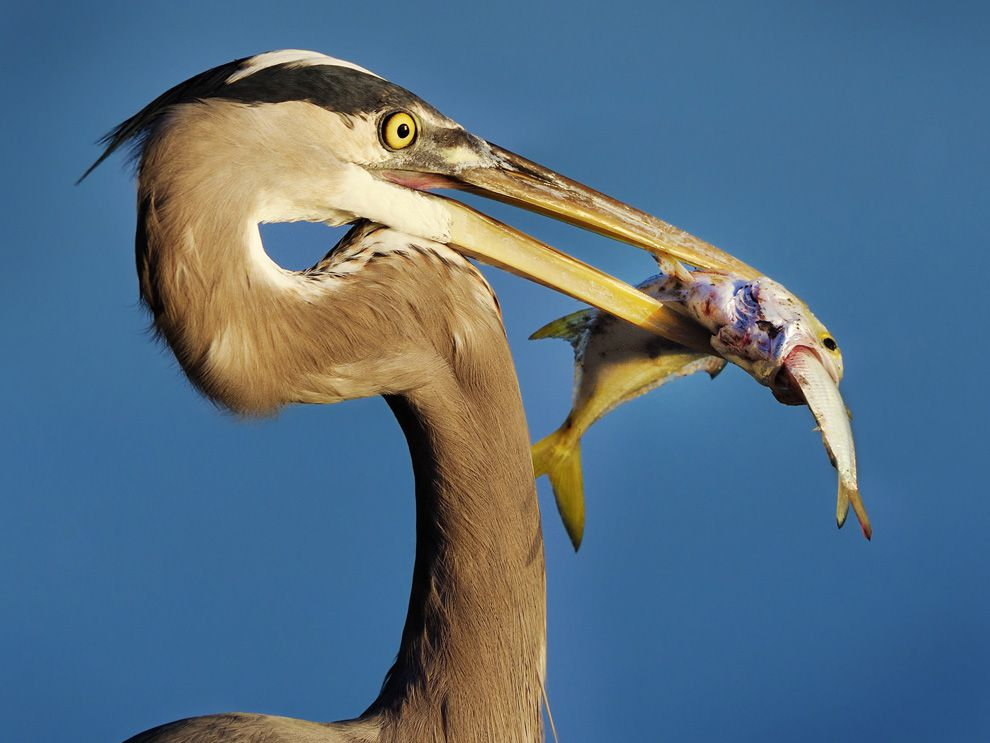
\includegraphics[width=0.8\textwidth]{food-chain}
  \end{columns}
\end{figure}
\end{frame}

\begin{frame}[fragile]{The good moves towards greater act}
  \begin{itemize}
  \item For something to be less than fully good is for it to have a privation; `evil' is the absence of an expected good.\vspace{5mm}
  \item A purely actual actualiser, being purely actual, can have no such privation.\vspace{5mm}
  \end{itemize}
\end{frame}


\begin{frame}[fragile]{Considerations}
  \begin{itemize}
  \item The Aristotelian argument for the `Unmoved Mover' grounds the transcendentals as realities.\vspace{5mm}
  \item There is no obvious way in which beauty classifies as a property of the transcendentals, unlike unity, truth and goodness. \vspace{5mm}
  \item Rather, it is the intelligence that recognises the\newline \emph{harmony} among parts --- a unity among diversity;\newline \emph{completeness} --- missing parts are perceived making a thing ugly;\newline \emph{brightness} of intelligibility --- fittingness to the knowing faculty.
  \end{itemize}
\end{frame}


\begin{frame}[plain]
  \titlepage
\end{frame}

\end{document}
